\section{Packaging Design}
\subsection{Overview}
Packaging for the \gls{ceenc} was constructed primarily from laser cut acrylic, as shown below. 
Laser cutting services were provided by Pokono, for a materials fee and machinery surcharge.
Design of the packaging was completed utilizing InkScape Vector Design Software.
Measurements were taken from the Master, Controller, and Driver boards, then translated into cutouts to support the components.
These cutouts were attatched to the sides of the enclosure, then stabilized by box joints \& machine screws.

\subsection{Design Considerations}
Cooling for the \gls{ceenc} is provided by two 40mm 5v Box Fans attatched to the back of the case.
They push air into the device, which allows egress only through the vents placed directly above the Motor Drivers.
This has the net effect of cooling all components, but with the primary focus on the Motor Drivers.
Interactive LCD components and Port Access was also added to the front and back.

\subsection{Material Selection}
Materials were chosen for both dimesnional stability, and aesthetic properties.
For the prototype unit, selection was limited to materials provided by the manufacturer.
Laser cut acrylic was used for the front and back of the enclosure, to allow for finer detail.
The acrylic chosen was also tinted, to allow for the LCD within the device to be visible when powered, but prevent the rest of the device from showing.
3-Ply laser cut walnut veneer was used for the sides of the enclosure.
This material is both structurally sound, and visually pleasing. 
Costs could be reduced here by choisng a less expensive mediums such as acrylic or cardboard.

\subsection{Cost Analysis}
Enclosure costs are primarily a result of the limited production quantity. 
Material costs for the entirety of the device are well below the \$10.00 mark, but manufacturing fees push the total cost above \$50.00.
Should the \gls{ceenc} be put into production, the total cost for the enclosure is expected to be below \$18.00.
This is calculated based upon laser cutting time cost estimates for large batches, and the existing material cost.
With the present design, full cutting of the enclosure takes between 5 and 10 minutes.
At the standard rate of $50.00 per machine hour, this translates to $8.00 per unit.
Additional costs incurred for processing, shipping, and technician time will not be incurred for larger orders.

\begin{figure}[h]
	\centering
	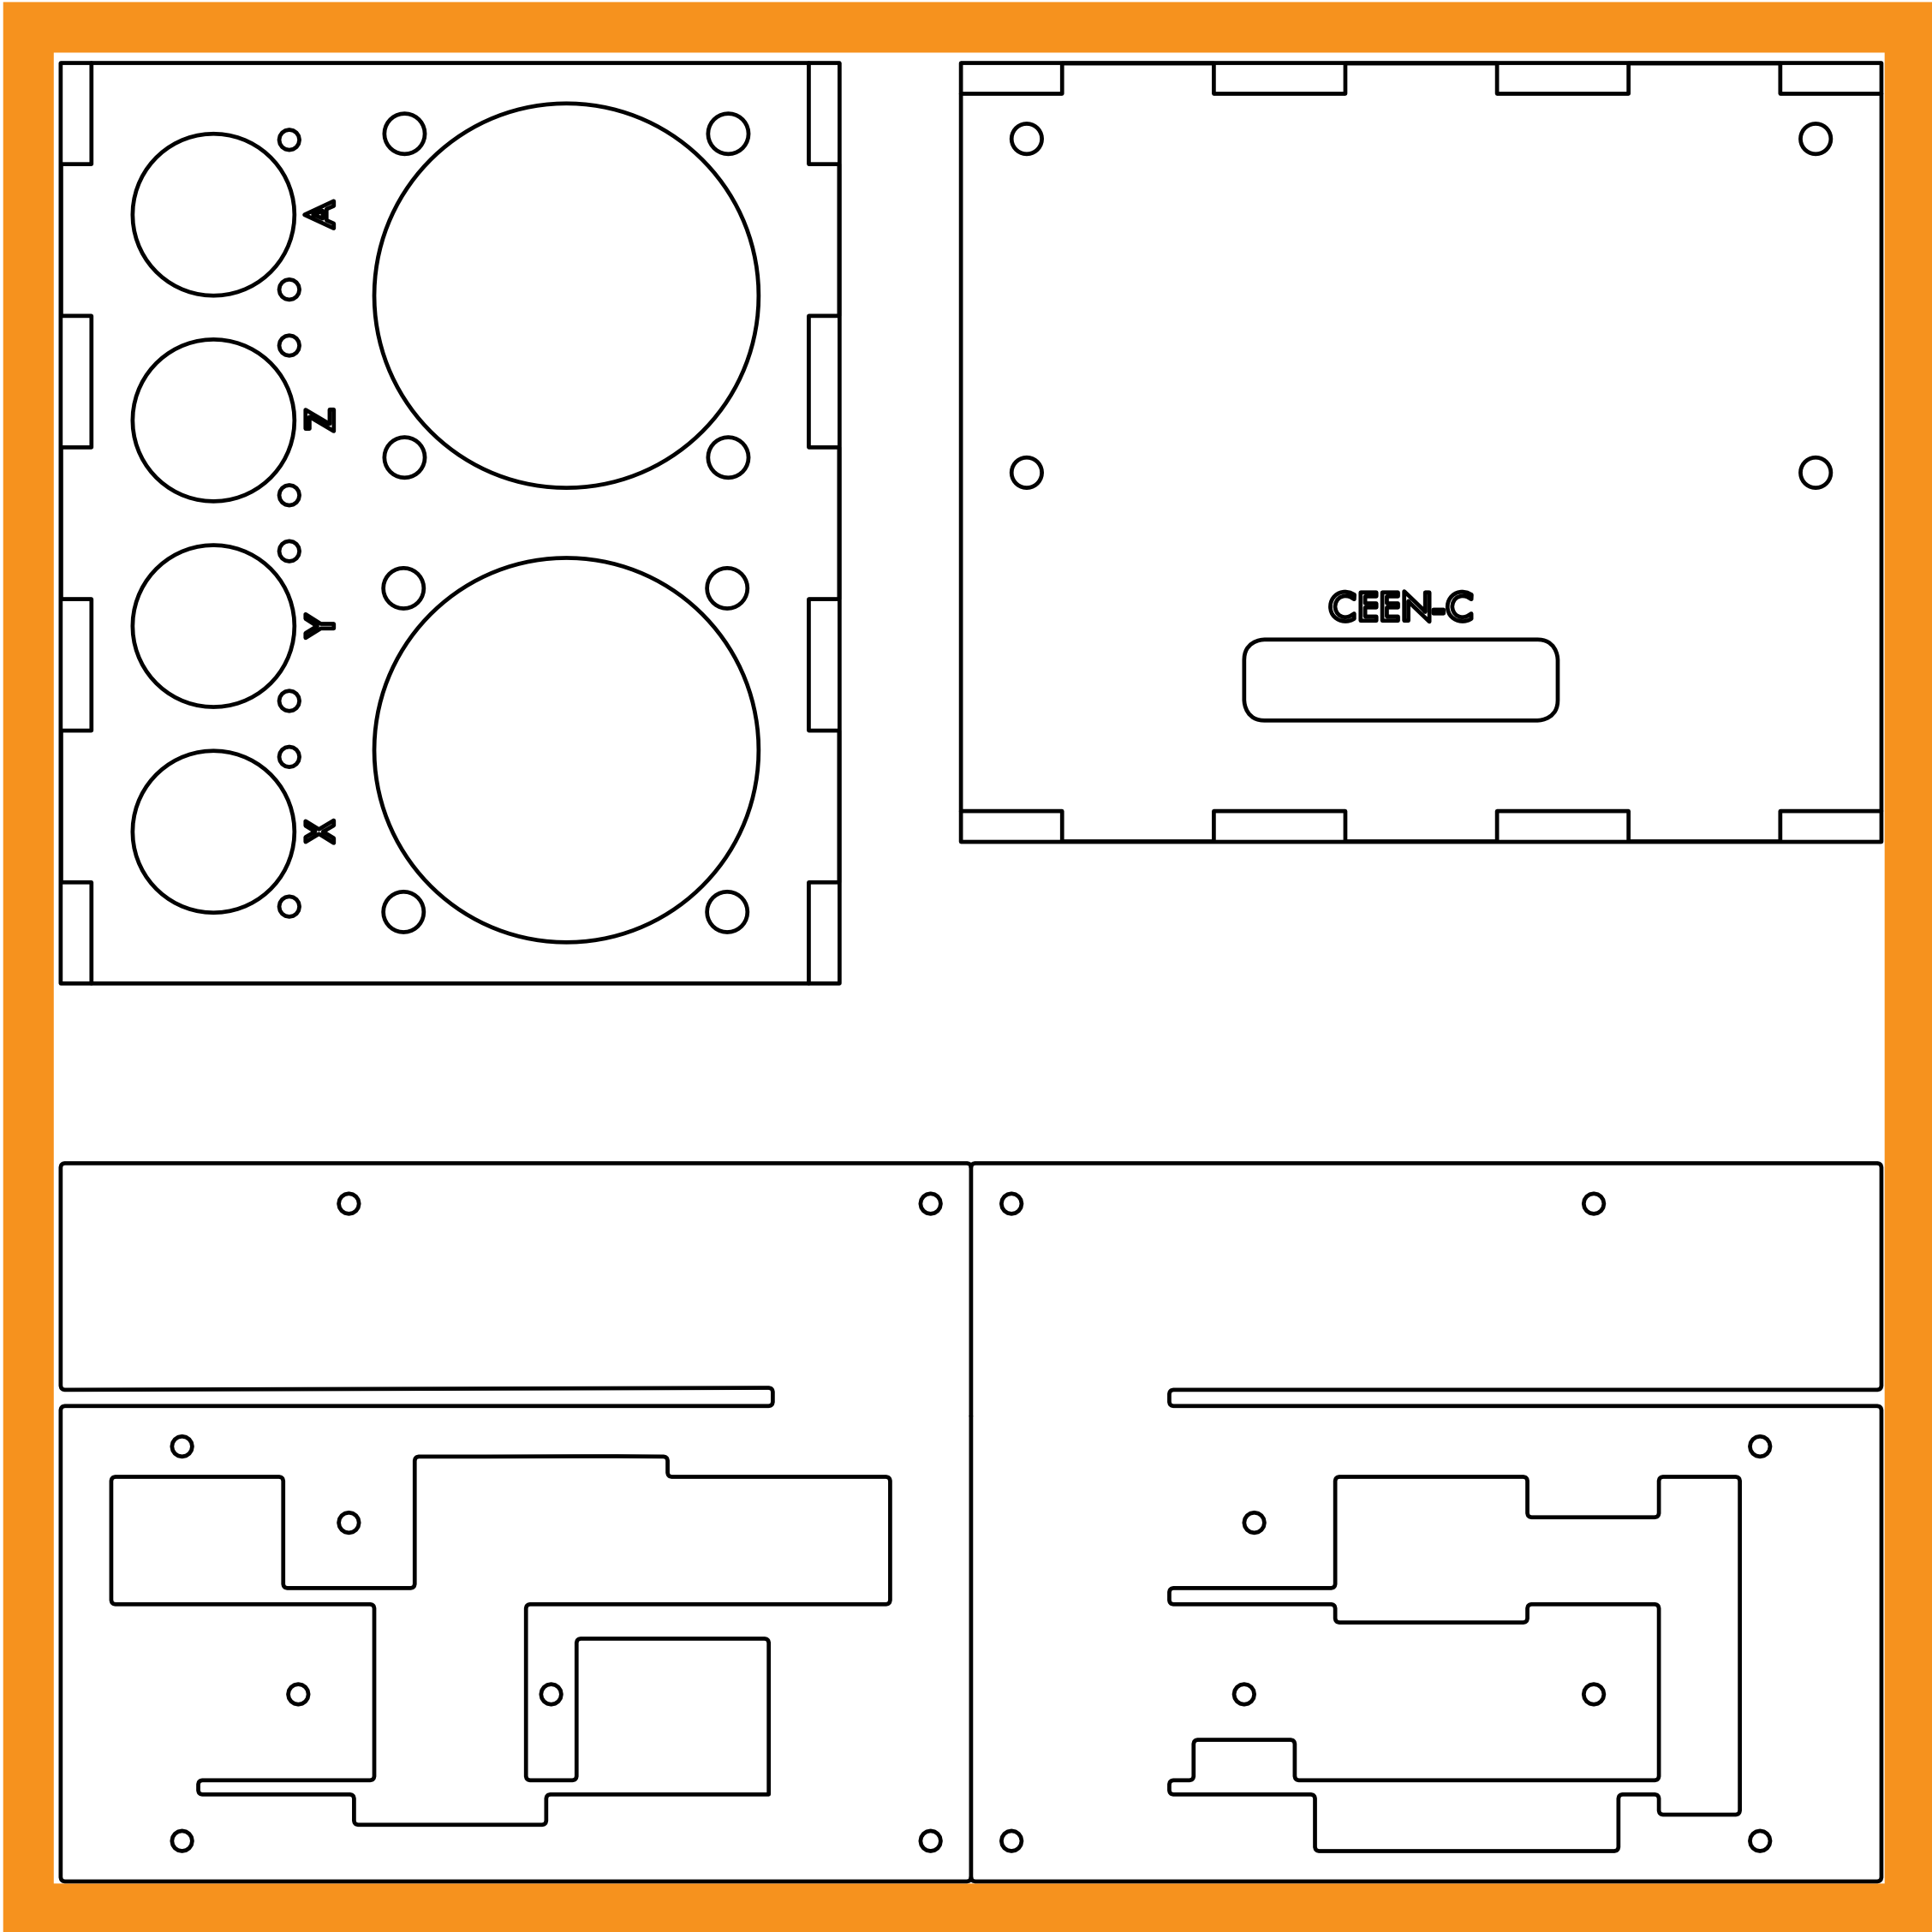
\includegraphics[width=1\textwidth]{packaging-design/front.png}
	\caption{Enclosure Front}
	\label{fig:front}
\end{figure}

\begin{figure}[h]
	\centering
	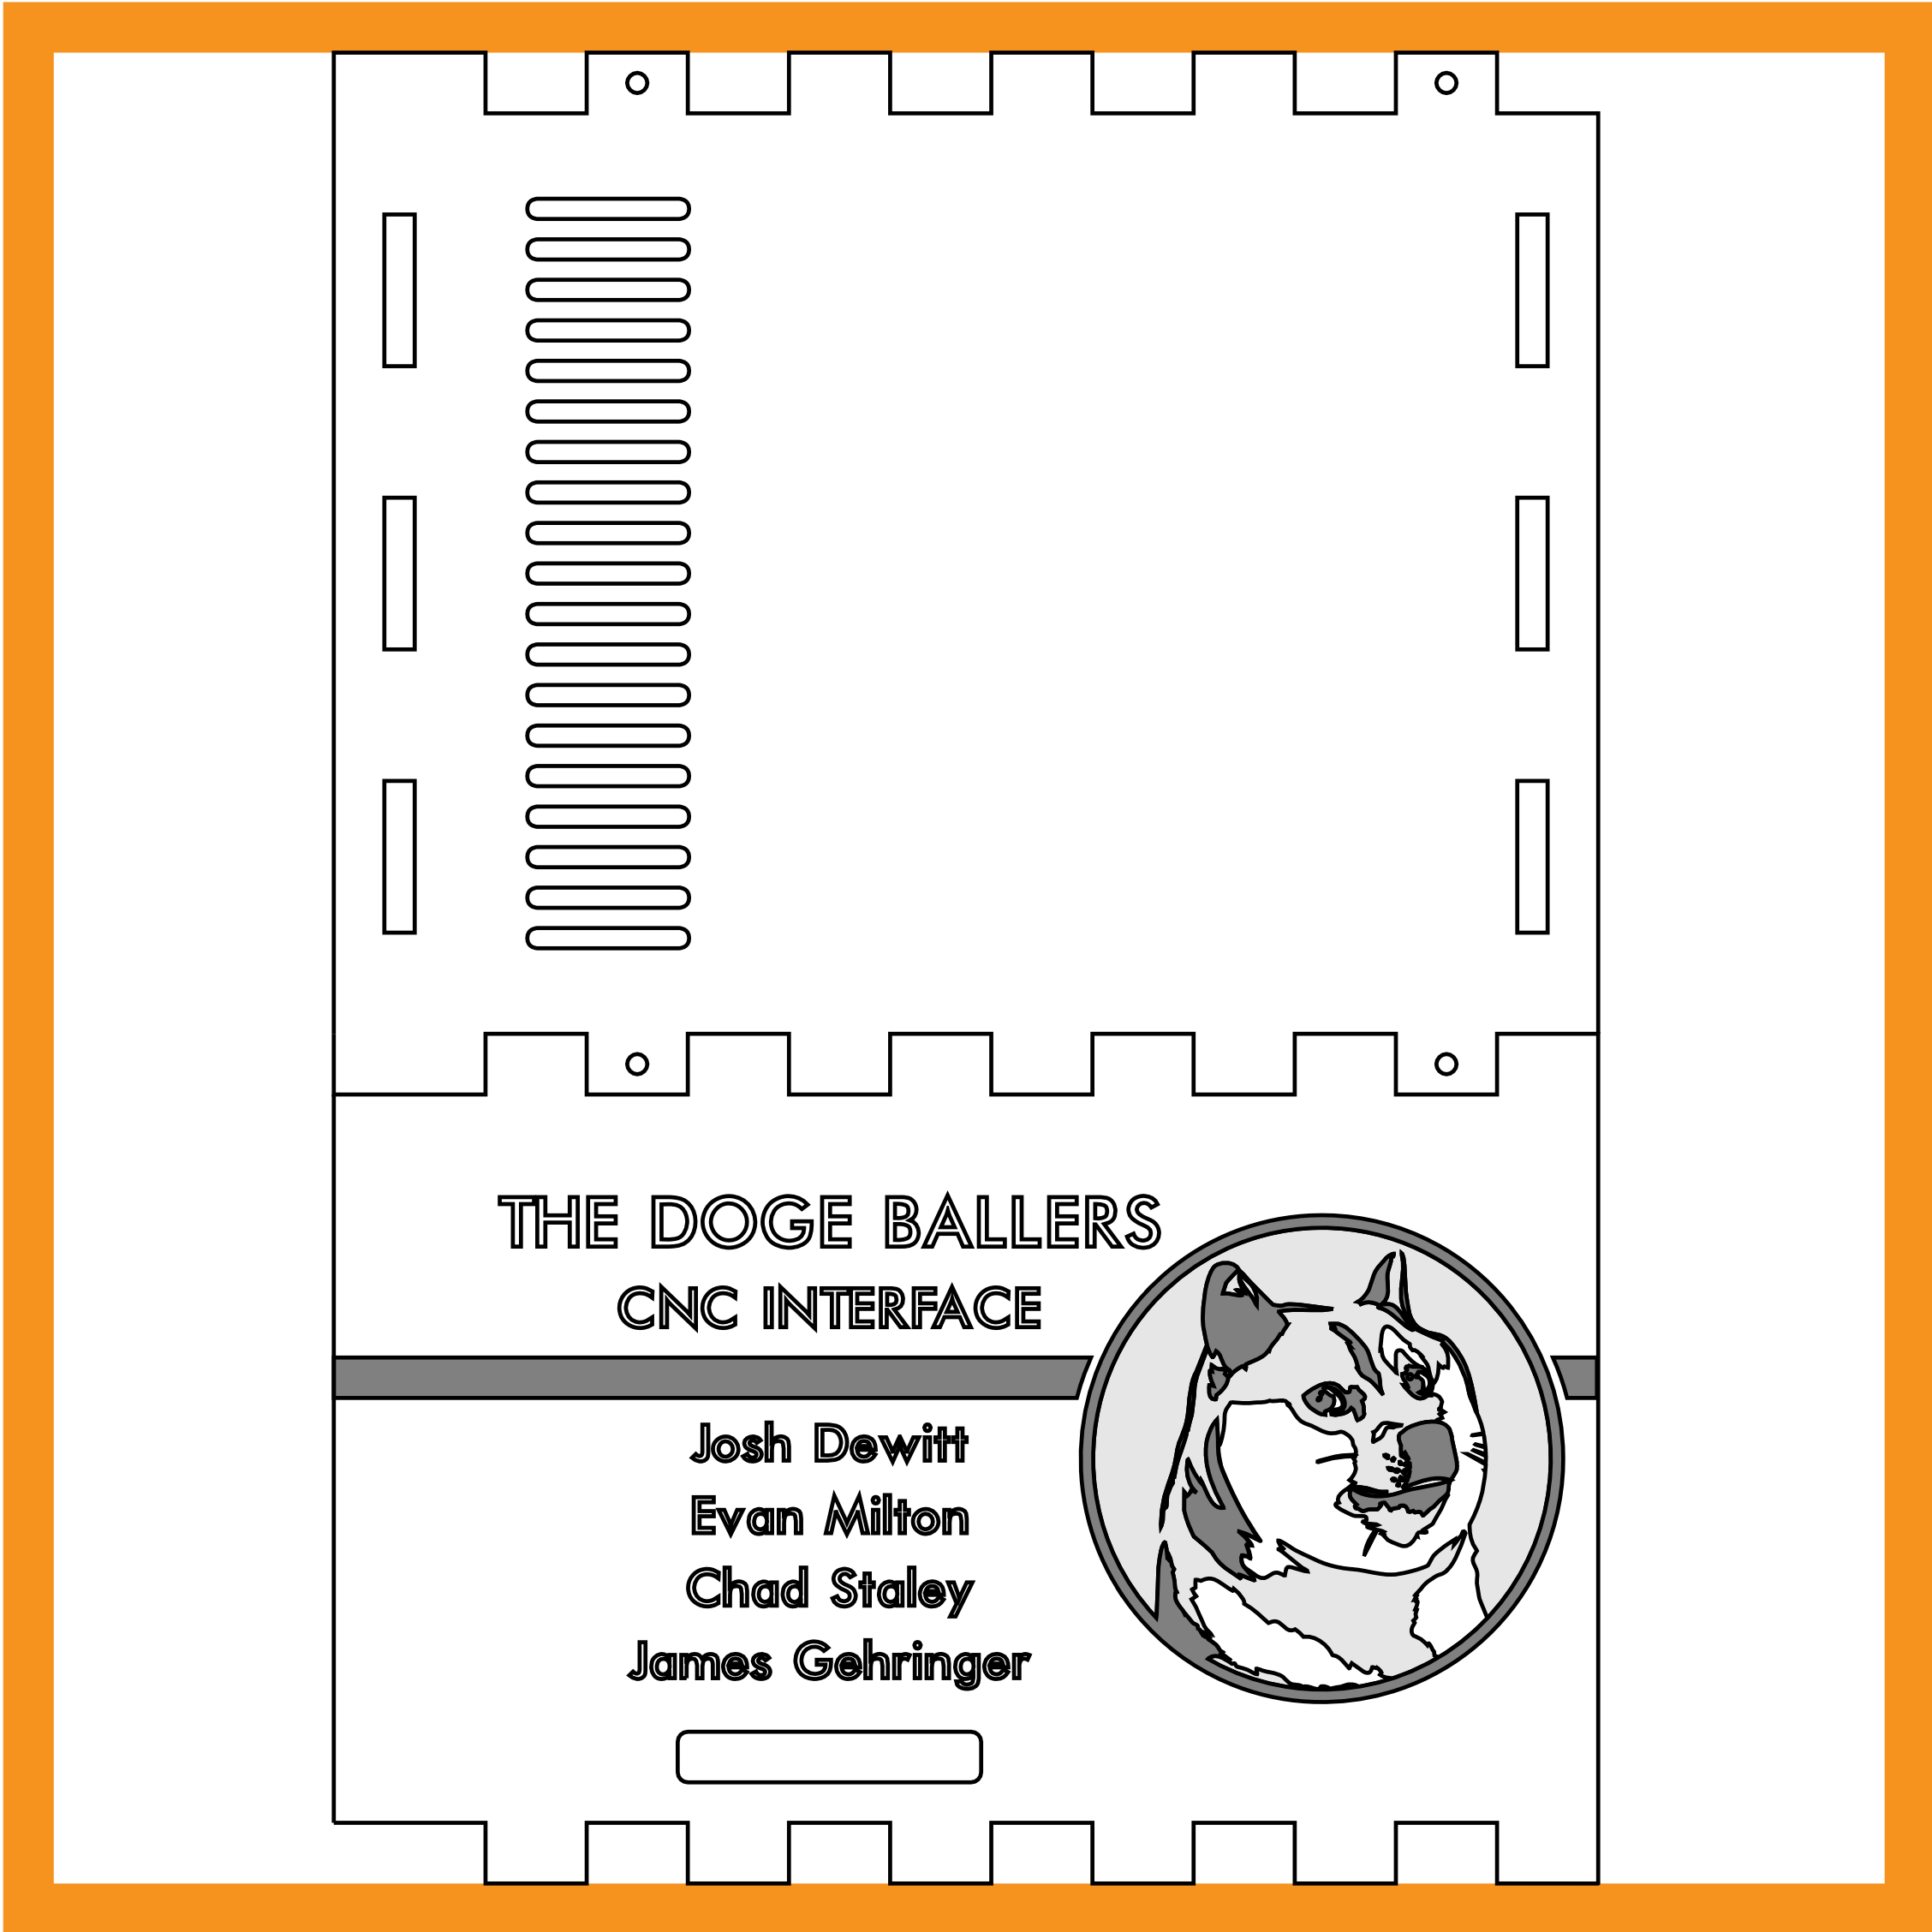
\includegraphics[width=1\textwidth]{packaging-design/side1.png}
	\caption{Enclosure Side Right}
	\label{fig:side1}
\end{figure}

\begin{figure}[h]
	\centering
	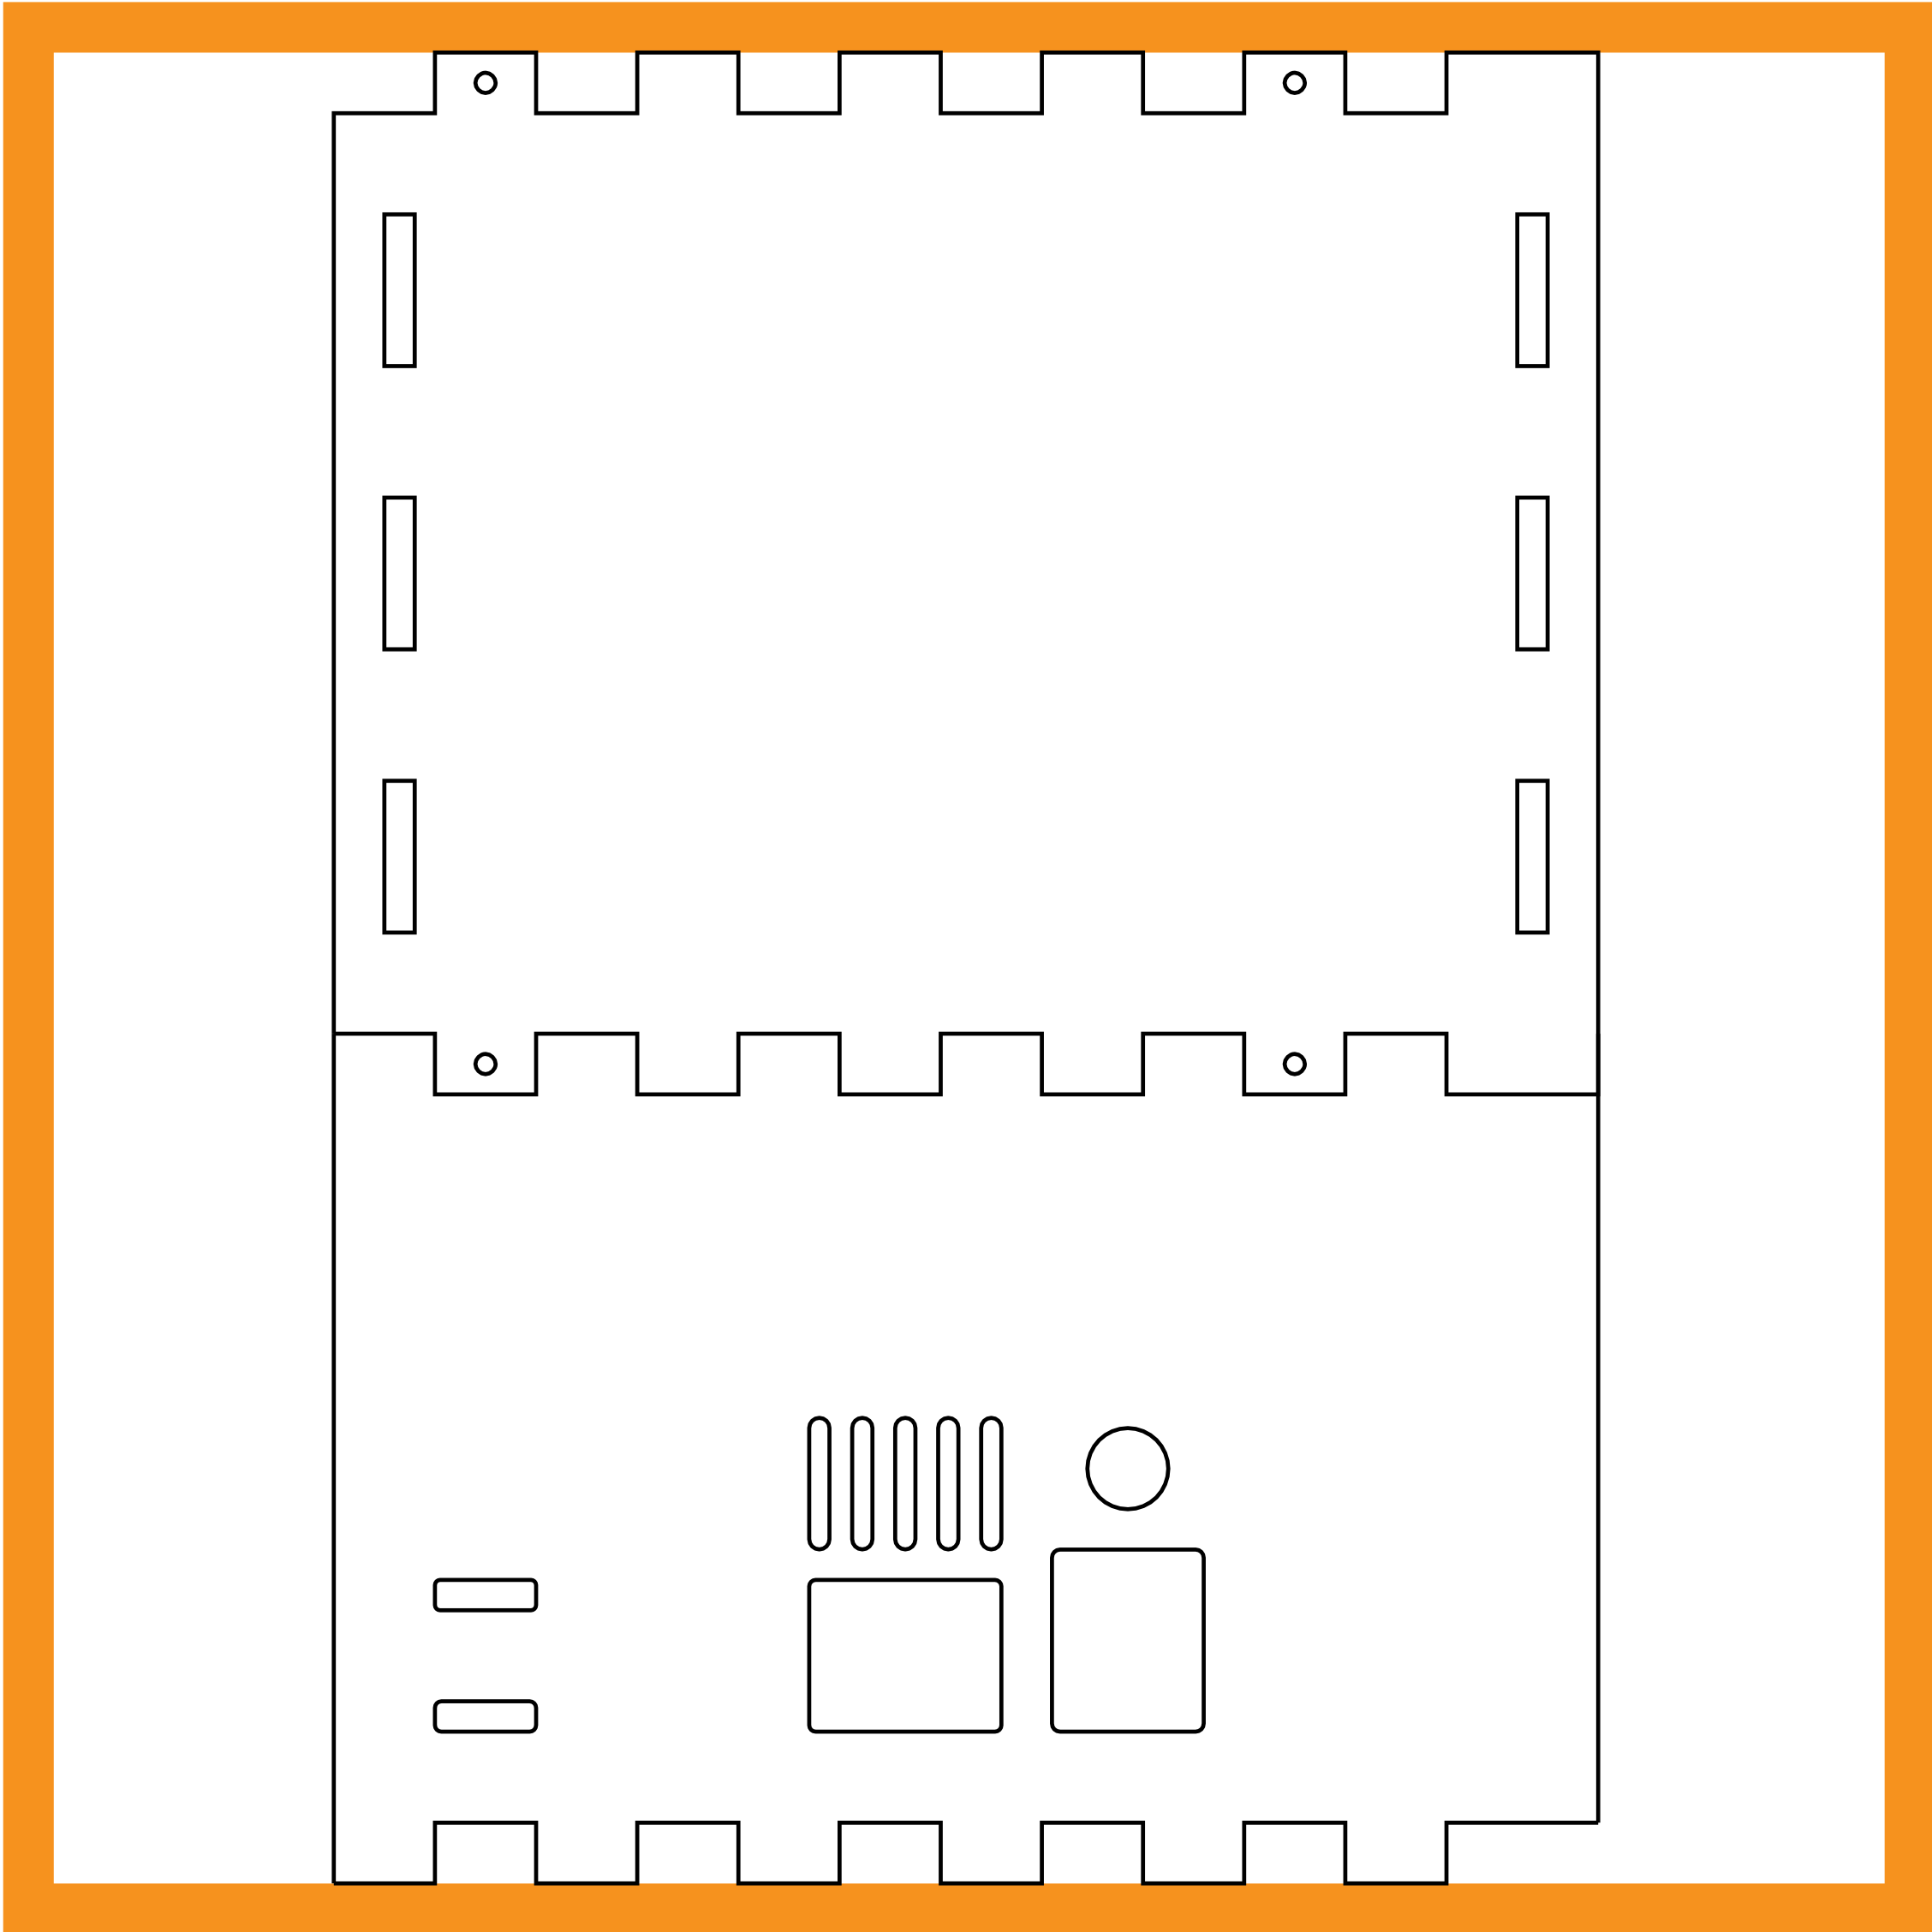
\includegraphics[width=1\textwidth]{packaging-design/side2.png}
	\caption{Enclosure Side Left}
	\label{fig:side2}
\end{figure}